\section{Empirical Results}\label{sec:results}

\section{Data}\label{subsec:data}
In the empirical analysis, we consider the risk reduction capability of the BTC-future (BTCF) on five cryptos
, BTC, ETH, ADA, LTC, and XRP, and five crypto indexes, BITX, BITW100, CRIX, BITW20, and BITW70,
For each of the 10 hedging portfolios, a crypto or index is considered as the spot and held in a unit size long position,
and the BTCF is held in short position of OHR unit in order to reduce the risk of the spot.
All the hedging portfolios are cross asset hedging except the BTCF portfolio.
ETH, ADA, LTC, and XRP are popular cryptos tradable in various exchanges and have large market capitalization.
BITX, BITW100, and CRIX are market-cap weighted crypto indexes with BTC as constituent.
BITX and BITW100 tracks the total return of the 10 and 100 cryptos with largest market-cap respectively.
CRIX decides the number of constituents by AIC and track that number of cryptos with largest market-cap.
In our case, the number of constituents in CRIX is 5.
BITW20 is also a market-cap weighted crypto index but with 20 largest market-cap cryptos outside the constituents of
BITX.
BITW70 has the same construction as BITW20 but with 70 largest market-cap cryptos outside BITX and BITW20.
Therefore, BTC is excluded as constituent in BITW20 and BITW70. \medskip

We collect the spots' and BTCF's daily price at 15:00 US Central Time (CT).
The reason of choosing this particular time is that the CME group determines the daily settlements for BTCFs based on the trading activities on CME Globex between 14:59 and 15:00 CT.
15:00 CT is also the reporting time of the daily closing price by the Bloomberg Terminal (BBT).
Cryptos data are collected from a data provider called Tiingo.
Tiingo aggregates crypto OHLC (open, high, low, and close) prices fed by APIs from various exhcanges.
Tiingo covers major exchanges, e.g. Binance, Gemini, Poloniex etc., so Tiingo's aggregated OHLC price is a good representation a market tradable price.
For each crypto, we match the opening price at 15:00 CT from Tiingo with the daily closing price of BTCF from BBT.
Since CRIX is not available at 15:00 CT, we recalculate a hourly CRIX using the monthly constituents weights and the hourly OHLC price data collected from Tiingo.
BITX, BITW20, BITW70, and BITW100 are collected from the official website of their publisher Bitwise.com.
The daily reporting time of the Bitwise indexes is 15:00 CT. \medskip

At the time of writing, the CRIX' is undergoing the listing process on the S\&P Dow Jones Indices,
the official CRIX data will then be calculated with Lukka Prime Data and available to public via S\&P.



















%\francis{\em This section is under construction}
%Cryptocurrenices are traded around the clock, but CME future are traded from
%Sunday to Friday from 05:00 p.m. to 04:00 p.m. U.S. central time.
%We match the timestamps and timezones of different data sources.
%
%
%\begin{table}[htbp]
%    \centering
%    \begin{tabularx}{\textwidth}{s|CCCCCCCC}
%      \hline\hline
%     \# & Asset & Data Source & Type & Tradable at CT\footnotemark & Tradable at CET\footnotemark during CST\footnotemark & Tradable at CET during CDT\footnotemark & Tradable at UTC during CST & Tradable at UTC during CDT\\       \hline
%      1 & Bitcoin & Coingecko API & Hourly Close &  & 11:00pm D+0 & 11:00pm D+0 & 10:00pm D+0$^*$ &10:00pm D+0$^*$ \\\hline
%      2 & CME Future & Bloomberg & Daily Open & 05:00pm D-1 & 00:00am D+0$^*$ & 00:00am D+0$^*$ & 11:00pm D-1 & 10:00pm D-1 \\       \hline
%      3 & CME Future & Bloomberg & Daily Close & 04:00pm D+0& 11:00pm D+0$^*$ & 11:00pm D+0$^*$ & 10:00pm D+0 & 09:00pm D+0\\       \hline
%      4 & CRIX & IRTG (from Coingecko) & Index &  &  &  & & 00:00am D+0$^*$\\\hline
%    \end{tabularx}
%    \caption{$^*$ indicates the timestamp of raw data from data source. }
%    \label{tab:table}
%\end{table}
%
%\addtocounter{footnote}{-3}
%\footnotetext{CT stands for U.S. Central Time. It represents two observances of time, the Central Standard Time (CST) and the Central Daylight Time (CDT)}
%\addtocounter{footnote}{1}
%\footnotetext{CET stands for Central European Time. It is one hour ahead UTC.}
%\addtocounter{footnote}{1}
%\footnotetext{CST is six hours behind UTC.}
%\addtocounter{footnote}{1}
%\footnotetext{CDT is five hours behind UTC.}
%
%Hedging Pair 1 is hedging \#1 (Bitcoin Spot) with \#3 (CME future).
%The time difference between the two prices is zero.
%They are both adjusted to CET time:
%\#1 by pandas.Series.dt.tz\_convert; \#3 by retrieving data from Bloomberg Terminal located in Berlin. \medskip
%
%Hedging Pair 2 is hedging \#4 (CRIX) with \#2 (CME future).
%We observe \#2 two hours and one hour before \#4 during CST and CDT respectively.
%
%
%\subsection{Time Difference}\label{subsec:time-difference}
%\begin{table}[h]
%    \centering
%
%\begin{tabular}{lrrrr}
%\toprule
%{} &     Open &     High &      Low &    Close \\
%\midrule
%2021-02-02 23:00 &  36360.0 &  38155.0 &  36240.0 &  37790.0 \\
%2021-02-01 23:00 &  34205.0 &  36665.0 &  34070.0 &  36535.0 \\
%2021-01-31 23:00 &  33715.0 &  35280.0 &  32800.0 &  34265.0 \\
%2021-01-28 23:00 &  33995.0 &  39530.0 &  32590.0 &  35180.0 \\
%2021-01-27 23:00 &  31005.0 &  33710.0 &  30350.0 &  33085.0 \\
%\bottomrule
%\end{tabular}
%       \caption{CME Bitcoin Future Raw Data}
%    \label{tab:table0} \medskip
%
%    \begin{tabular}[width=\textwidth]{llrrrr}
%\toprule
% &                      date &           CRIX &   future &  log return CRIX &  log return future \\
%\midrule
%0 & 2021-02-04  &  104518.468839 &  38080.0 &         0.054757 &           0.046220 \\
%1 & 2021-02-03  &   98949.179255 &  36360.0 &         0.059741 &           0.061097 \\
%2 & 2021-02-02  &   93210.948461 &  34205.0 &         0.002204 &           0.014429 \\
%3 & 2021-02-01  &   93005.711051 &  33715.0 &         0.013628 &          -0.008271 \\
%4 & 2021-01-29  &   91746.863103 &  33995.0 &         0.081917 &           0.092065 \\
%\bottomrule
%    \end{tabular}
%    \caption{CRIX \#4 with Opening price of CME Bitcoin future \#2 and their log returns}
%    \label{tab:table2} \medskip
%
%\begin{tabular}{llrrrr}
%\toprule
%{} &                      date &           CRIX &   future &  log return CRIX &  log return future \\
%\midrule
%0 & 2021-02-05  &  103348.488555 &  38220.0 &        -0.011257 &           0.011314 \\
%1 & 2021-02-04  &  104518.468839 &  37790.0 &         0.054757 &           0.033774 \\
%2 & 2021-02-03  &   98949.179255 &  36535.0 &         0.059741 &           0.064146 \\
%3 & 2021-02-02  &   93210.948461 &  34265.0 &        -0.016175 &          -0.026353 \\
%4 & 2021-01-30  &   94730.919657 &  35180.0 &         0.032007 &           0.061398 \\
%\bottomrule
%\end{tabular}
%    \caption{CRIX \#4 with Closing price of CME Bitcoin future \#3 shifted for one day (D-1) and their log returns}
%    \label{tab:table3}
%\end{table}
%
%\clearpage
%\begin{figure}[ht]
%    \centering
%    \includegraphics[scale=.35]{_pics_notes/CRIX_future_Open_Close.pdf}
%    \end{figure}
%
%Kendall's tau between CRIX and future Close is 0.608429;\\
%Kendall's tau between CRIX and future Open is 0.673266; we pick this unless we have hourly CRIX.
%
%\subsection{Statistics of Percentage Difference Between CME Bitcoin future Open Price and Last Close Price}
%
%$$\text{diff} = \frac{\text{Open}_{t} - \text{Close}_{t-1}} {\text{Close}_{t-1}}$$
%
%Mean of diff = 0.00236\\
%Std of diff = 0.02206\\
%Max of diff = 0.16394 \\
%UQ of diff = 0.00814 \\
%Median of diff = 0.00132\\
%LQ of diff = -0.00412 \\
%Min of diff = -0.12190 \\

\begin{figure}[!th]
\centering
\begin{minipage}[t]{.475\textwidth}
    \centering
    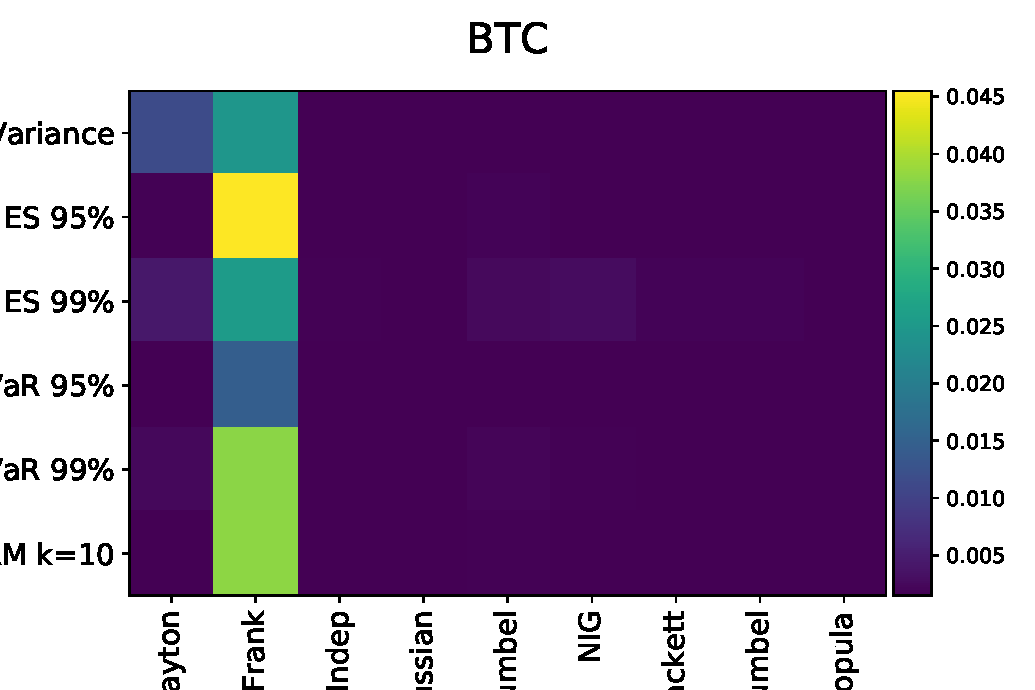
\includegraphics[width=\textwidth]{_pics/MSE_BTC.pdf}
  \caption{Mean square errors of BTC-BTCF portfolios constructed with different copula and risk minimization objectives.
    The Frank copula is inferior in the BTC-involved portfolios.
    \href{http://www.quantlet.com/}{\includegraphics[height=\baselineskip]{_pics/qletlogo_tr.png}} }
\label{fig:MSE_BTC}
\end{minipage}%
\hfill
\begin{minipage}[t]{.475\textwidth}
    \centering
    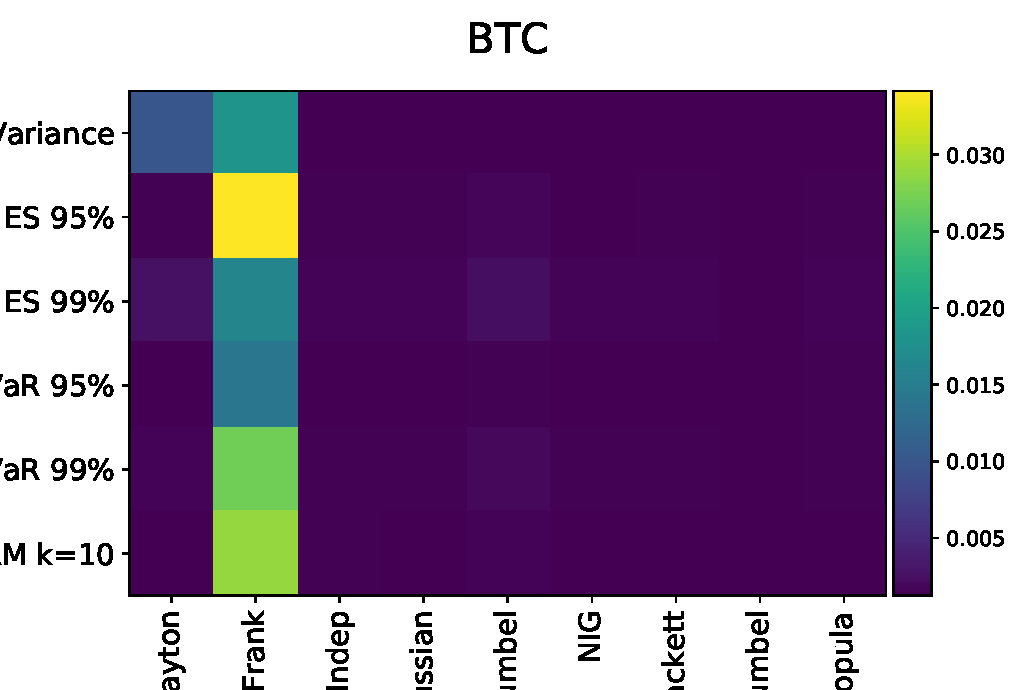
\includegraphics[width=\textwidth]{_pics/semiLowerVariance_BTC.pdf}
  \caption{Lower semivariance of BTC-BTCF portfolios constructed with different copula and risk minimization objectives.
  The Frank copula is obviously inferior.
  \href{http://www.quantlet.com/}{\includegraphics[height=\baselineskip]{_pics/qletlogo_tr.png}} }
\label{fig:SLV_BTC}
\end{minipage}
\end{figure}
\subsection{An overview of the hedged portfolios without the copula selection step}\label{subsec:HP1}
First, we analyse the results of hedged portfolios without the copula
selection step in order to get a better understanding of how a copula
affects the hedged portfolio with various risk minimization
objectives.
To do so, we inspect the hedge performance of copulas by
the mean square error and lower semi-variance.
The mean square error
is the distance between a perfect hedge and the hedged portfolio
returns $\operatorname{MSE}= \mbox{\sf E} (R^2)$.
The lower semi-variance is defined as 
$\operatorname{LSV}=\mbox{\sf E} \{R-\mbox{\sf E}(R)^2\}1(R\leq \mbox{\sf E}(R))$.
All results presentedd here are out-of-sample results obtained without
the copula selection step in order to compare the performances across
copulae.

\newpage
\begin{figure}[!]
        \centering
        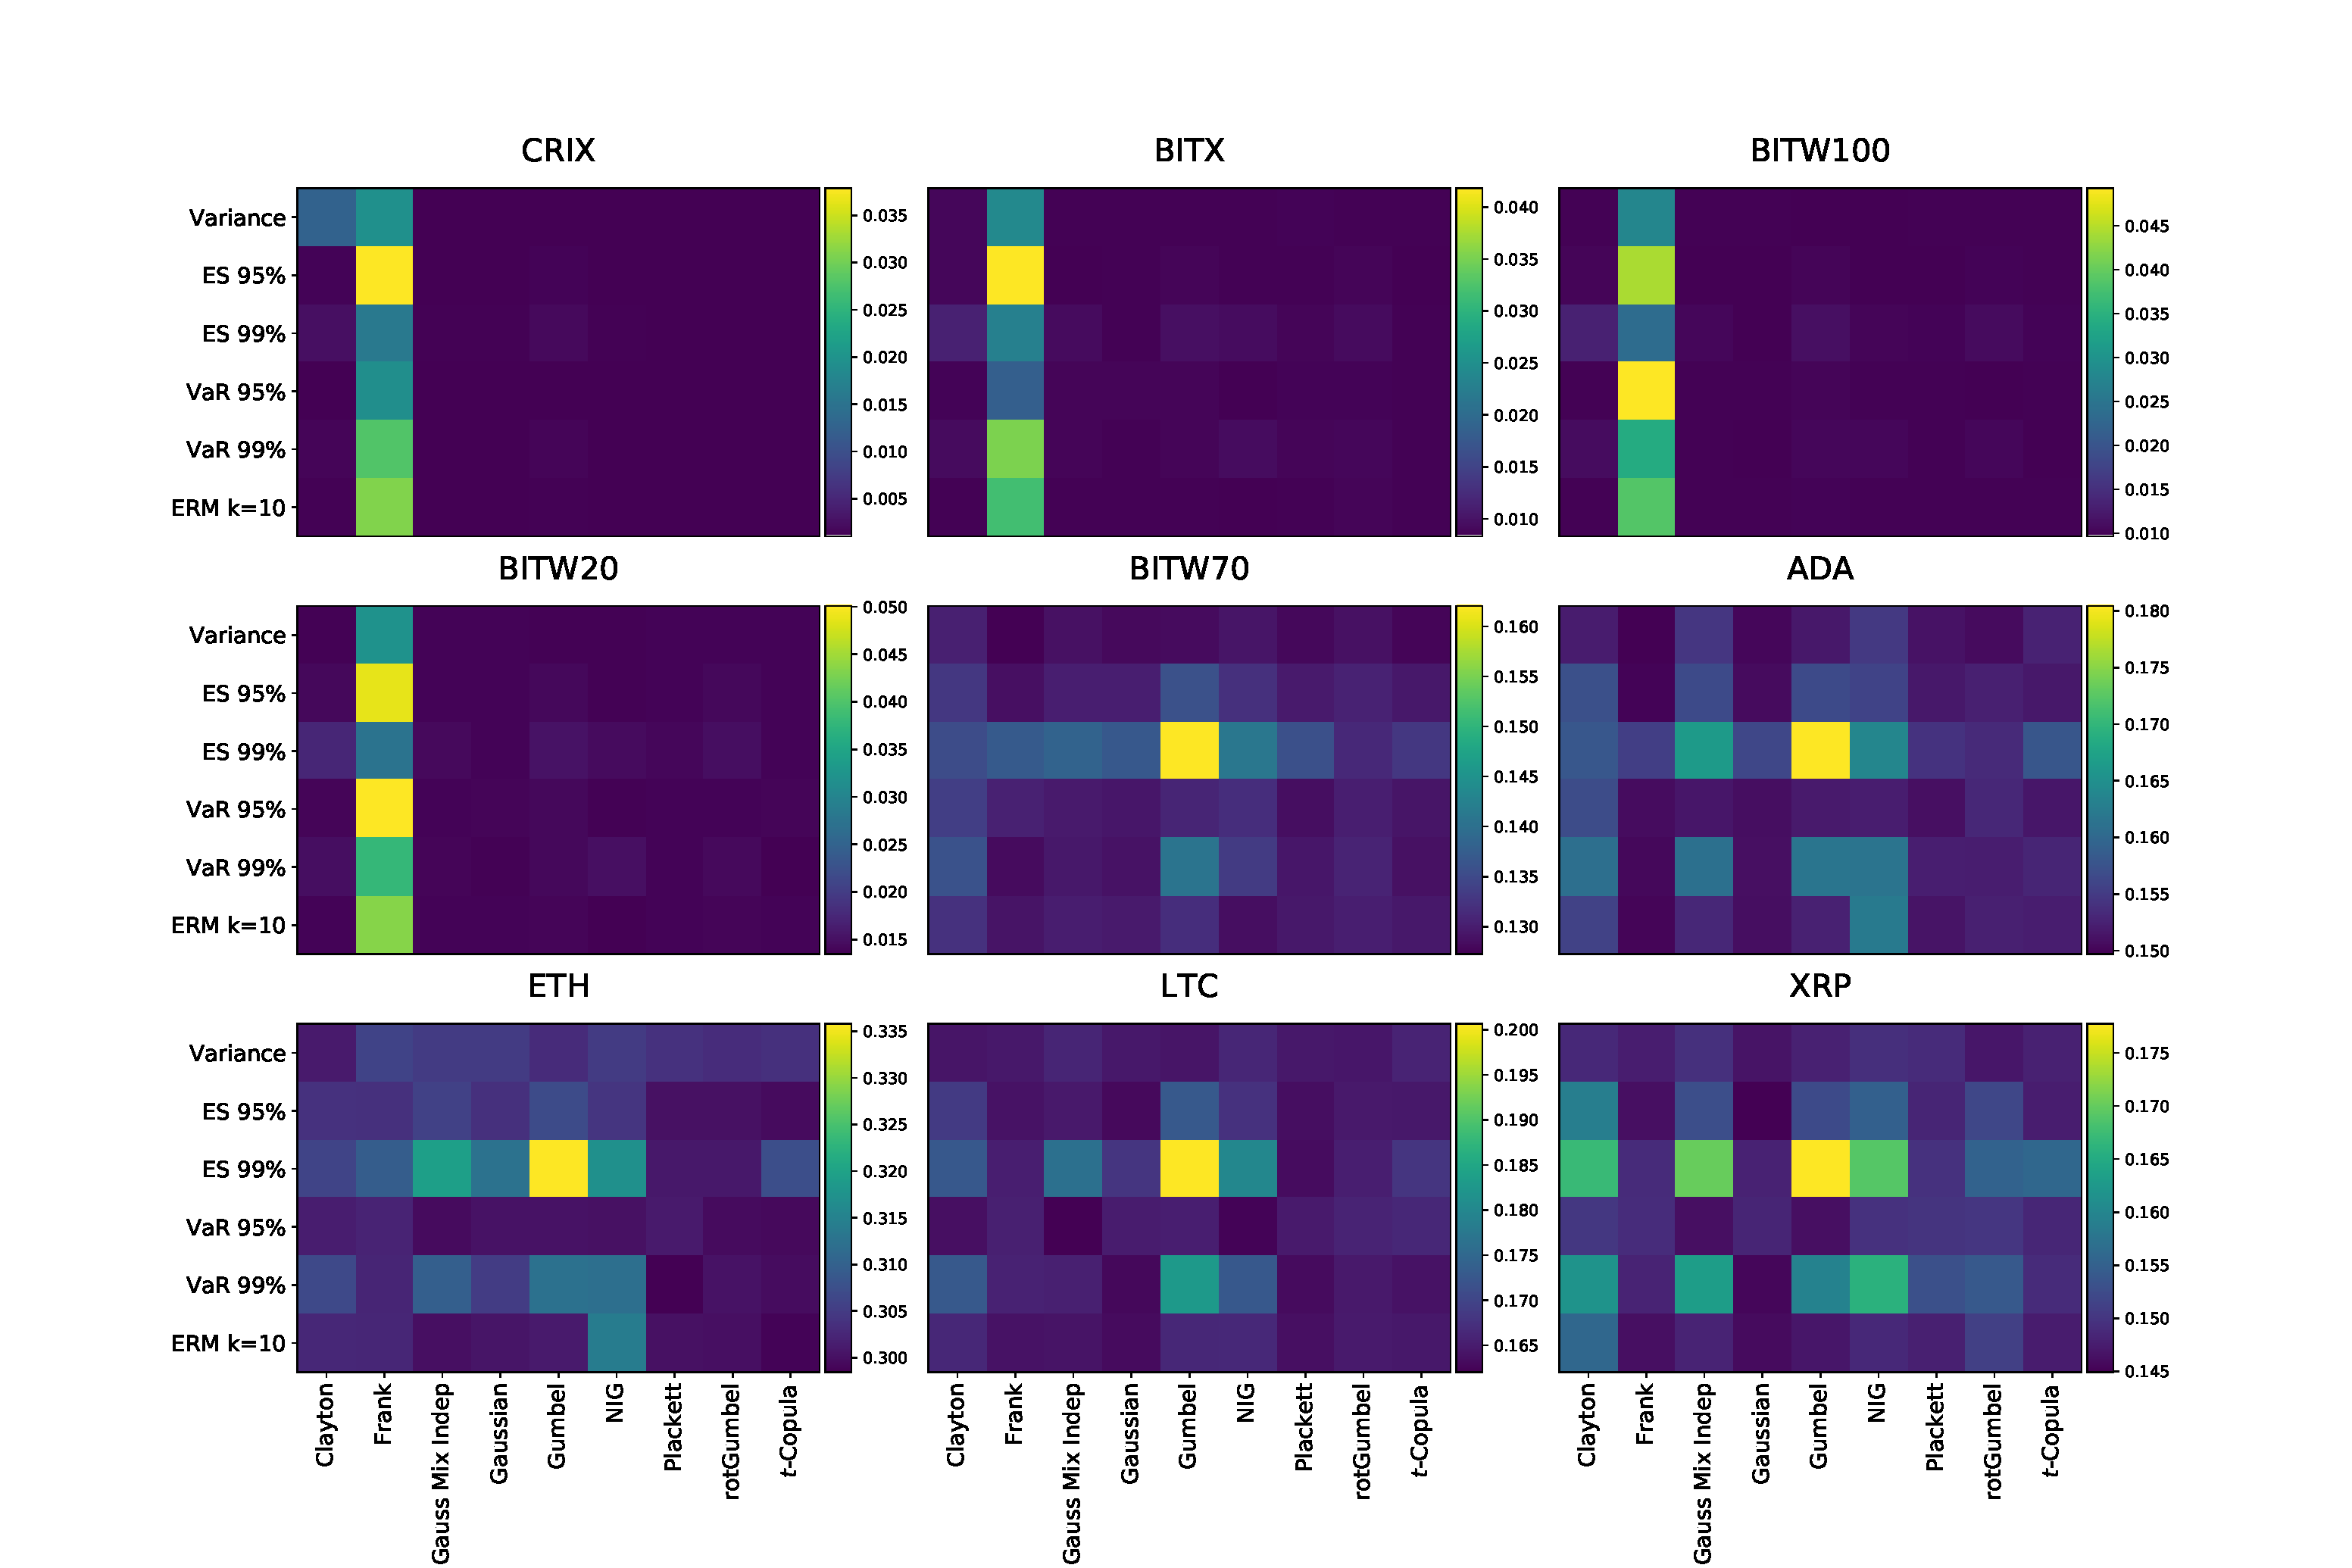
\includegraphics[width=\textwidth]{_pics/MSE_other.pdf}
      \caption{Mean square errors of portfolios constructed with different copula and risk minimization objectives.
      \href{http://www.quantlet.com/}{\includegraphics[height=\baselineskip]{_pics/qletlogo_tr.png}} }
    \label{fig:MSE_other}
%\end{subfigure}%
%\end{figure}

%\begin{figure}[!]
%\begin{subfigure}{\textwidth}\centering
        \centering
        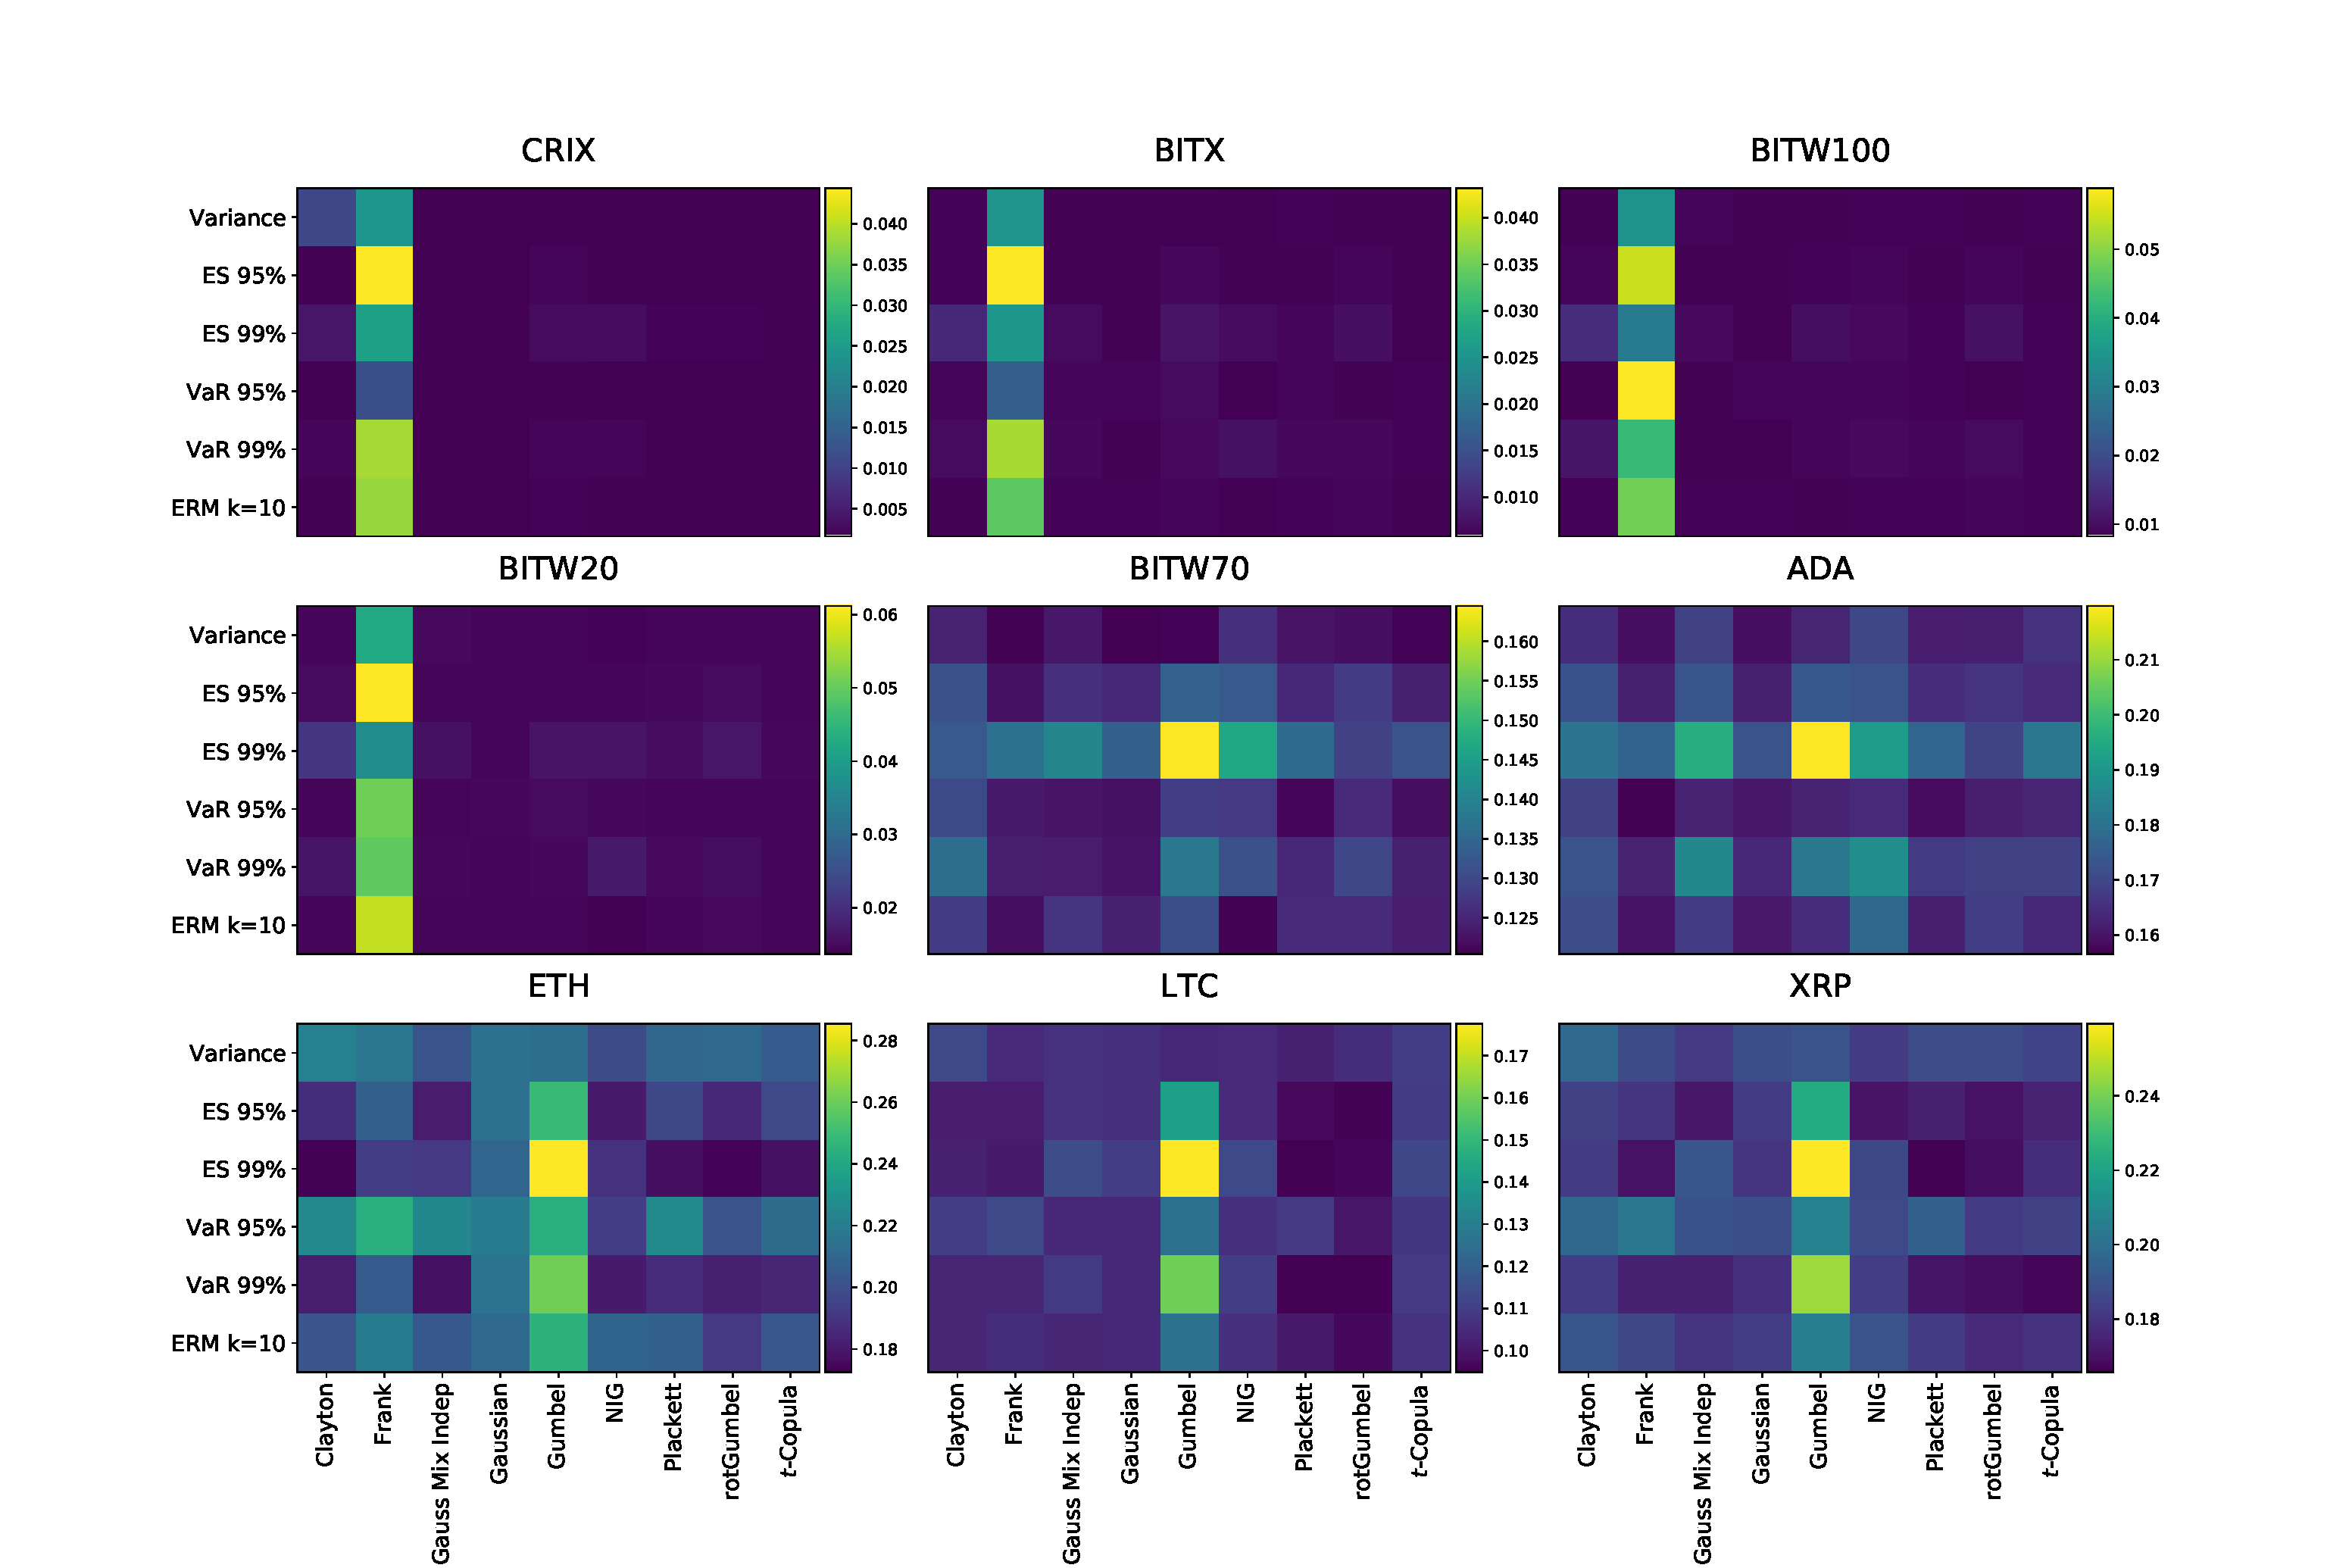
\includegraphics[width=\textwidth]{_pics/semiLowerVariance_other.pdf}
      \caption{Lower semivariance of portfolios constructed with different copula and risk minimization objectives.
      \href{http://www.quantlet.com/}{\includegraphics[height=\baselineskip]{_pics/qletlogo_tr.png}}
        \natp{\em [Just wondering if it's an option to streamline the axis,
    so we can also see the differences in performance for the
    different portfolios?]}
  }
    \label{fig:SLV_other}
\end{figure}
\clearpage

%\textcolor{darkblue}{As presented in Fig 3 and 4, either individual cryptos or indice, their cumulative returns dropped in Mar 2020. it's due to the result of COVID19. we can explain this for these two plots.}\\
%\textcolor{darkblue}{Here i think it should insert a paragraph to interpret how you enter the copulae, otherwise it's weird that comes to Fig 5 and 6.}\\

Figure \ref{fig:MSE_BTC} and \ref{fig:SLV_BTC} \natp{\em [reduce size
  of figures]} are the mean square
error and lower semivariance of BTC-BTCF. We can see that the Frank copula
is the worst performing copula: 
the resulting hedged portfolio returns is far away from a perfect
hedge. \natp{\em [I think I did the plots on a log-scale to see some
  more detail. Can you try this? Or would you like me to do this?]}
In Figures \ref{fig:MSE_other} and \ref{fig:SLV_other}, the phenomenom
of Frank copula being inferior to its counterparts can be observed
from the results of the CRIX, BITX, BITW100, and BITW20-BTCF
portfolios. 
Interestingly, the spot in those portfolios usually have a strong
dependence with the BTCF. 
In contrast, the inferiority of the Frank copula is less prominent in
the BITW70, ADA, ETH, LTC and XRP-BTCF portfolios. 
We suspect that the Frank copula is not a choice to model assets with
strong dependence. \textcolor{darkblue}{The Frank copula is not
  appropriate for data that exhibit asymmetric and heavy tails.}
\natp{\em [It is mentioned earlier that the Frank copula has no tail
  dependence. This would explain that a strong dependence in finance
  cannot be modelled well, as we observe strong dependence in
  particular in the tails.]}

We can also observe from Figures \ref{fig:MSE_other} and
\ref{fig:SLV_other} that theGumbel copula is not performing as well as 
other copulas in the ETH, LTC, and XRP-BTCF portfolios. 
The reason is the Gumbel copula has only upper tail dependence,
while the ETH, LTC, and XRP exhibit lower tail dependence with BTCF. 
We will discuss this in the following section. \natp{\em [Please avoid
  the term ``dependency'', use dependence.]}

\subsection{Copula Selection Results}\label{sec: copula results}
\begin{table}[t]
 \ra{1.1}
    {\begin{tabularx}{\textwidth}{lYYYYY} \toprule
         Copula/Asset & $t$ & Plackett & GMI & rotGumbel & NIG \\ \midrule
     \multicolumn{6}{l}{Individual Cryptos}                                                                                 \\
        \ \ \ BTC          & 73         & 4                 & 2                        & 1                  & 31                  \\
        \ \ \ ETH          & 3          & 6                 & 8                        & 94                 & 1                   \\
        \ \ \ ADA          & 0          & 0                 & 0                        & 0                  & 112                 \\
        \ \ \ LTC          & 13         & 0                 & 3                        & 32                 & 64                  \\
        \ \ \ XRP          & 0          & 31                & 3                        & 78                 & 0                   \\
   \multicolumn{6}{l}{Crypto Indices with BTC Constituent}                                                                  \\
        \ \ \ BITX         & 39         & 0                 & 14                       & 16                 & 12                  \\
        \ \ \ CRIX         & 47         & 0                 & 11                       & 3                  & 27                  \\
        \ \ \ BITW100      & 42         & 0                 & 8                        & 29                 & 2                   \\
    \multicolumn{6}{l}{Crypto Indices without BTC Constituent}                                                              \\
        \ \ \ BITW20       & 0          & 0                 & 0                        & 78                 & 3                   \\
        \ \ \ BITW70       & 0          & 0                 & 0                        & 80                 & 1                   \\
    \bottomrule
    \end{tabularx}
        \caption{Copula Selection Results. }









    \label{tab:copulasection}
\end{table}
\textcolor{darkblue}{Interpret the steps of copula selection.} \\
Next, we inspect the copula selection result.
Although the copula selection is only an intermediate step to obtain the OHRs,
the result of this step can help us better understand the dependence
feature between BTCF and the assets we study in this work.
This gives us valuable information to model the assets in the future.
Decisions of the AIC procedure are summarised in Table \ref{tab:copulasection}.

Overall, the $t$-copula, rotated Gumbel (rotGumbel), and the NIG
factor copula are the most frequently chosen copulae by the AIC
procedure.

The $t$-copula is frequently chosen to model the dependence between
the BTC and BTC-involving-indices, CRIX, BITX, BITW100, and the BTC
future.
BTC and BTC-involving-indices exhibit strong (upper and lower) tail
dependence with BTCF.  We interpret tail dependence as a strong
tendency for one asset to be extreme when another is extreme and
vice versa \citep{McNeil2015}.
In fact, the $t$ copula has been suggested in various empirical
studies to model financial data, such as~\cite{zeevi2002beyond} and~
\cite{breymann2003dependence}.
Those studies suggest that the $t$-copula is a better model compared
to the Gaussian copula as financial data typically exhibit heavy tails
and tail dependence. \textcolor{darkblue}{(because the thick and left
  skew  properties of financial data tail distribution are documented. )}
\medskip

On the other hand, the radial symmetry of the $t$-copula appears to be
a poor choice to model the remaining hedging pairs.
\cite{demarta2005t} describe the symmetry feature ``strong'', because if
$(U_1, ..., U_d)$ is a vector distributed in $t$-copula,
then $(U_1, ..., U_d) \overset{\mathcal{L}}= (1-U_1, ...,
1-U_d)$. \natp{\em [Just to be clear: is that not the definition of
  radial symmetry? If so, call it definition, and place it earlier
  where the term is used for the first time.]}
This symmetry can be justified in the dependence structure between a
futures and its underlying by the theory of futures pricing,
which suggests the price of a futures is a function of the underlying
price \citep{hull2003options}.
However, there is no such relationship between a futures and an asset
which is not the underlying, and so the radial symmetry becomes a
drawback to model other hedging pairs e.g. ETH and BITX70.
Another drawback of the $t$-copula is the lack of flexibility to model
off-diagonal region since $\rho$ and $\nu$ jointly control the density
of the off-diagonal region.
%The off-diagonal region (HF paper breymann2003dependence)
This is why sometimes the Gaussian Mix Independence (GMI) better model
the dependence.  \natp{\em [I would suggest to shorten this. The
  argument might be more concise if explaining that crashes take place
  in all coins and indices simultaneously (this should be backed by
  the Figures above), whereas positive development is more
  idioosyncratic.]}

Among the three popular copulae, rotGumbel copula shows its ability to model the dependency between ETH and BTCF,
94 out of 112 training sets are best fitted with the rotated Gumbel.
rotGumbel also performs well when modelling dependency between XRP, BITW20, BITW70, and the BTCF.
In particular, the whole time series of the two indices, BITW20 and BITW70, are best fitted solely with the rotated Gumbel copula.
The frequently chosen rotated Gumbel indicates the styled fact of
financial data: prices tends to drop together.  \natp{\em [No need to
  repeat what's already in the table. Rather, if there are insights,
  then state them, otherwise it is OK to also say nothing.]}

In fact, Clayton's AIC in many of the training sets is the second lowest, just higher than that of rotated Gumbel.
This is because the Clayton copula has the same ability to model the lower quantile dependence.
However, Clayton's radial like feature does not match the behaviour of
the financial data. \medskip

It is worth to mention that although the NIG factor copula is penalised heavily due to its three parameters setup,
it is frequently chosen to be the best copula to model the dependency
between individual cryptos and the BTC future.
An extreme case would be ADA, where only NIG factor is chosen in our dataset.
Another dependence structure being best described by the NIG factor
copula is the pair of LTC-BTCF, with
64 out of 112 training sets best fitted by the NIG factor copula.
Indices like BITX and CRIX are sometimes best fitted with the NIG
factor copula as well, accounting for modelling 12 and 27 training
sets respectively.
The popularity of the NIG factor reflects the ability of the copula to
model very complex dependence structure: the
NIG factor copula is able to model the tail, radial asymmetry, and
off-diagonal behaviour. \natp{\em [What do you mean by
  ``off-diagonal behaviour''?]} \medskip

The Frank copula is generally not a good choice to model financial
data (as also reported by \cite{barbi2014copula}).
Plackett is characterised by its dependence parameter being equal to
the cross-product ratio % \citep{joe1997multivariate}
. \natp{\em [Provide
  reference to Equation (32).]}
However, apparently, this property does not capture the dependence
structure of cryptos and BTCF.

\natp{\em [until here]}

\subsection{Hedged portfolios with the copula selection step}\label{subsec:HP2}
\begin{table}[t] \centering
    %\begin{table}[!] \centering
\resizebox{.75\textwidth}{!}{%
\begin{tabular}{lcccccc}
\toprule
{} &    Mean \% &      Std \% &    Skew &    Kurt &       MD \% & Date of MD\\
\midrule
Variance &  0.0215 &  0.3221 & -1.0119 &  3.1929 & -0.0144 &  2020-11-30 \\
VaR 95\%  &  0.0253 &  0.3294 & -0.9725 &  3.4373 & -0.0153 &  2020-11-30 \\
VaR 99\%  &  0.0176 &  0.3270 & -1.0405 &  3.3742 & -0.0157 &  2020-11-30 \\
ES 95\%   &  0.0204 &  0.3234 & -1.0150 &  3.4423 & -0.0156 &  2020-11-30 \\
ES 99\%   &  0.0148 &  0.3476 & -0.8354 &  3.3054 & -0.0162 &  2020-11-30 \\
ERM k=10 &  0.0223 &  0.3221 & -1.0008 &  3.4153 & -0.0152 &  2020-11-30 \\
\bottomrule
\end{tabular}}
\caption{Summary statistics of BTC-BTCF hedge portfolios out-of-sample daily returns under different risk minimisation objectives.}
\label{tab:BTCrh}
%\end{table}
    \caption{Summary statistics of BTC-BTCF hedge portfolios out-of-sample daily returns under different risk minimisation objectives.}
\label{tab:BTCrh}
\end{table}
Table~\ref{tab:BTCrh} presents the summary statistics, maximum drawdown (MD) and the date of MD of the BTC-BTCF hedge portfolios.
The index column indicates the risk minimization objectives.
We observe that the statistics of the portfolios with different objectives are similar to each other.
The means of the returns are close to zero;
Standard deviations ranges from 0.32\% to 0.35\%;
Skewnesses are slightly negative (skew to the right);
Kurtosises are slightly larger than 3;
The MDs are close to zero and the date of MDs are 2020-11-30.

For the other spots, tables~\ref{tab:var_rh} to table~\ref{tab:ERM_rh} summarise the statistics
of daily returns of hedged portfolios.
The tables look repeating so we place them in the appendix.
For each hedge portfolios,
the first four moments as well as the maximum drawdown (MD) and the date of MD are very similar across different risk minimization objectives. \medskip
%This is because the optimal hedge ratios of different risk minimization objectives fall into a small range. \medskip

On the other hand, the statistics vary across spots.
Unsurprisingly, the BTC-involved spots, i.e. BTC, CRIX, BITX, and BITW100, are well hedged by the BTCF regardless of risk minimization objective.
Contrarily, BTC-not-involved spots' portfolios are less promising.
Th hedged portfolio returns are as volatile as the spots.
We will further discuss the effectiveness of hedge in the next section. %\ref{sec: HE results}.

\subsection{Hedging Effectiveness Results}\label{sec: HE results}
\begin{figure}[t]
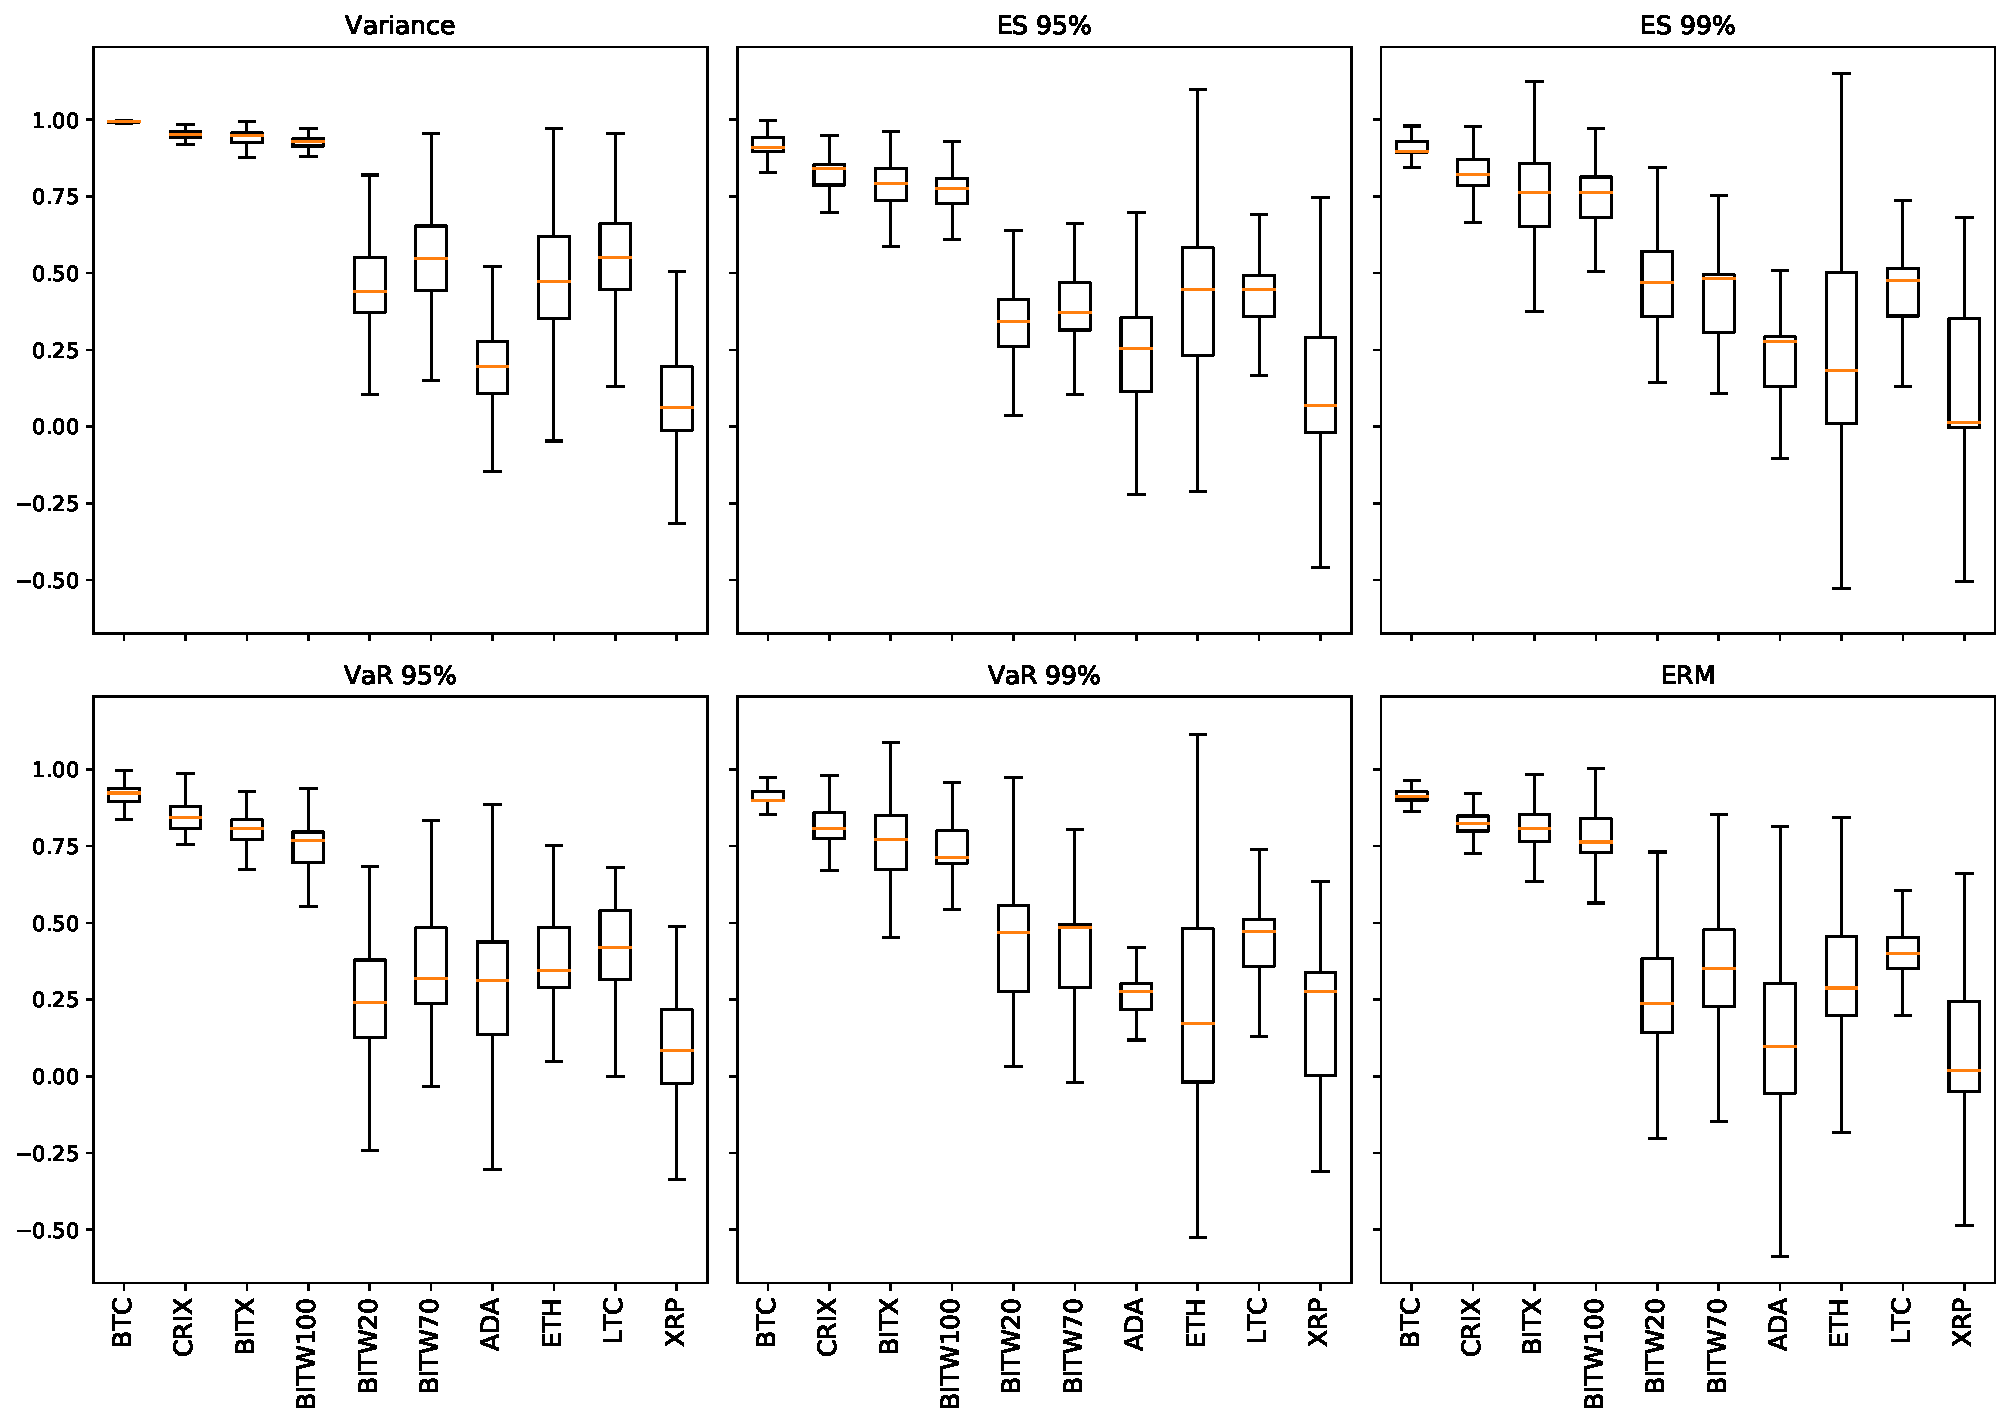
\includegraphics[width=\textwidth]{_pics/ES5_HE_boxplot.pdf}
  \caption{Hedging effectiveness (HE) of portfolios with different risk minimizatio objectives evaluated by the corresponding risk minimization objectives.
            The boxplots indicate the the median, upper quartile, lower quartile, minimium and maximum of the bootstrapped HE.
            The HE of BTC-involved spots are significantly higher than that of BTC-not-involved spots.
  \href{http://www.quantlet.com/}{\includegraphics[height=\baselineskip]{_pics/qletlogo_tr.png}} }
\label{fig:HEboxplot}
\end{figure}
In this section, we analyse the out-of-sample hedging effectiveness (HE) of BTCF as hedging.
HE is defined as $$\text{HE} = 1-\frac{\rho_h}{\rho_s},$$
a measure of the percentage reduction of portfolio risk attribute, in our case the spot $\rho_s$,
to hedged portfolio risk attribute $\rho_h$.
A higher HE indicates a higher hedging effectiveness and larger risk reduction. \medskip

The HE above is a generalisation of Ederington measure of hedging performance, where we,
in addition to variance, include other risk measures: Expected Shortfall 5\% and 1\% (ES5 and ES1), Value-at-Risk 5\% and 1\% (VaR5 and VaR1), and ERM.
In particular, ES5 is recommended by the Basel Committee on Banking Supervision (BCBS) to replace VaR as a quantitative risk metrics system.
The proposed reform aimed at enhancing the risk metric system's ability to capture tail risk. \medskip
%Discussions of the issue can be found in literatures.
%
We obtain a time series of out-of-sample $r^h$ of each hedging pair and each risk reduction objective by concatenating the out-of-sample results.
Then, we apply stationary block bootstrapping (SB) to the time series introduced by \cite{Politis1994} in our analysis in order to preserve the temporal structure of the data while sampling.
The SB procedure is as follow.
Assume a time series with $N$ observations $\{X_t\}_{t \in [1,N]}$ is a strong stationary, weakly dependence time series of interest,
we form blocks of samples $B = \{X_i, ..., X_{i+j-1}\}$.
Index $i$ is a random variable uniformly distributed over $[1,2,...,N]$ and $j$ is geometric distributed random variable with parameter .
The block index $i$ and block length $j$ are independent.
For any index $k$ which is greater than $N$, the sample $X_k$ is defined to be $X_{k(\mod N)}$.
For each block, we calculate the hedging effectiveness with different risk measures mentioned above.
We choose $p=0.005$, implying the expected block length is 200.
100 blocks are drawn for each risk minimising objective and spot. \medskip

From figure \ref{fig:HEboxplot}, we report, as expected, the BTC involving spots, the BTC, CRIX, BITX and BITW100, are well hedged by the BTCF.
The performances are consistent across different risk reduction objectives and different HE evaluation.
The median HE to BTC generated by various risk reduction objectives is ranging from 89.45\% to 99.31\%, median HE to CRIX is ranging from 81.13\% to 95.22\%,
median HE to BITX is ranging from 79.06\% to 94.84\%, median HE to BITW100 Is ranging from 71.07\% to 92.98\%. \medskip

The HE of BTCF to other cryptos and indices are substantially lower than to the BTC involving spots, but the consistency the performances across different risk reduction objectives and HE evaluation remains.
The median HE to BITW20 generated by various risk reduction objectives is ranging from 24.67\% to 47.02\%, median HE to BITW70 is ranging from 23.61\% to 49.30\%,
median HE to ADA is ranging from 9.01\% to 29.30\%, median HE to ETH Is ranging from 30.07\% to 36.18\%, median HE to LTC Is ranging from 37.74\% to 51.30\%,
median HE to XRP Is ranging from 0.46\% to 30.89\%.



%%% Local Variables:
%%% mode: latex
%%% TeX-master: "SRM"
%%% End:
